\section{Introduction}\label{sec:intro}

Federated learning is a decentralized machine learning approach that enables multiple clients to collaboratively train a shared model without exposing their private data \citep{mcmahan2017communication}. In this paradigm, each client independently trains a local model using its own data and subsequently sends the model updates to a central server. The server then periodically aggregates these updates to improve the global model until it reaches convergence. There are two primary settings in FL: cross-silo and cross-device \citep{kairouz2021advances}. Cross-silo FL typically involves large organizations (small number of clients), where most clients actively participate in every round of training \citep{chen2021bridging,lin2020ensemble}. In contrast, cross-device FL focuses on scenarios like smartphones (huge number of clients, e.g., millions), where only a limited number of clients participate in each round \citep{li2020federated,reddi2020adaptive}, due to communication bandwidth, client availability, and other issues. This paper primarily focuses on the cross-device setting with partial client participation since we discover and then solve its unique challenge ---``\textbf{\textit{period drift}}''.

Distinguished from traditional distributed optimization, the statistical heterogeneity of data has been acknowledged as a fundamental challenge in FL \citep{li2020federatedb,chen2021bridging,lin2020ensemble}. This data heterogeneity refers to the violation of the independent and identically distributed (non-iid) data assumption across clients, which can result in poor convergence and performance degradation when using \fedavg. \textit{Client drift} is recognized as one of the factors contributing to this issue and attracts numerous efforts to address it \citep{karimireddy2021scaffold,li2020federated,reddi2020adaptive}. This phenomenon is characterized by clients who, after multiple local updates, progress too far towards minimizing their local objective, consequently diverging from the shared direction. However, in cross-device FL, a different form of drift exists and could be more detrimental to the training process than client drift, which has not been extensively studied. \textit{This drift occurs periodically as different clients participate in each communication round, and these participating clients as a group may exhibit distinct data distribution that deviates from the overall distribution of all clients.} 
Period drift is fundamentally different from the noise in SGD, as further described in Appendix~\ref{appdx:analogy}. \looseness-1

\begin{wrapfigure}{r}{0.55\textwidth}
   \vspace{-3mm}
   \centering
   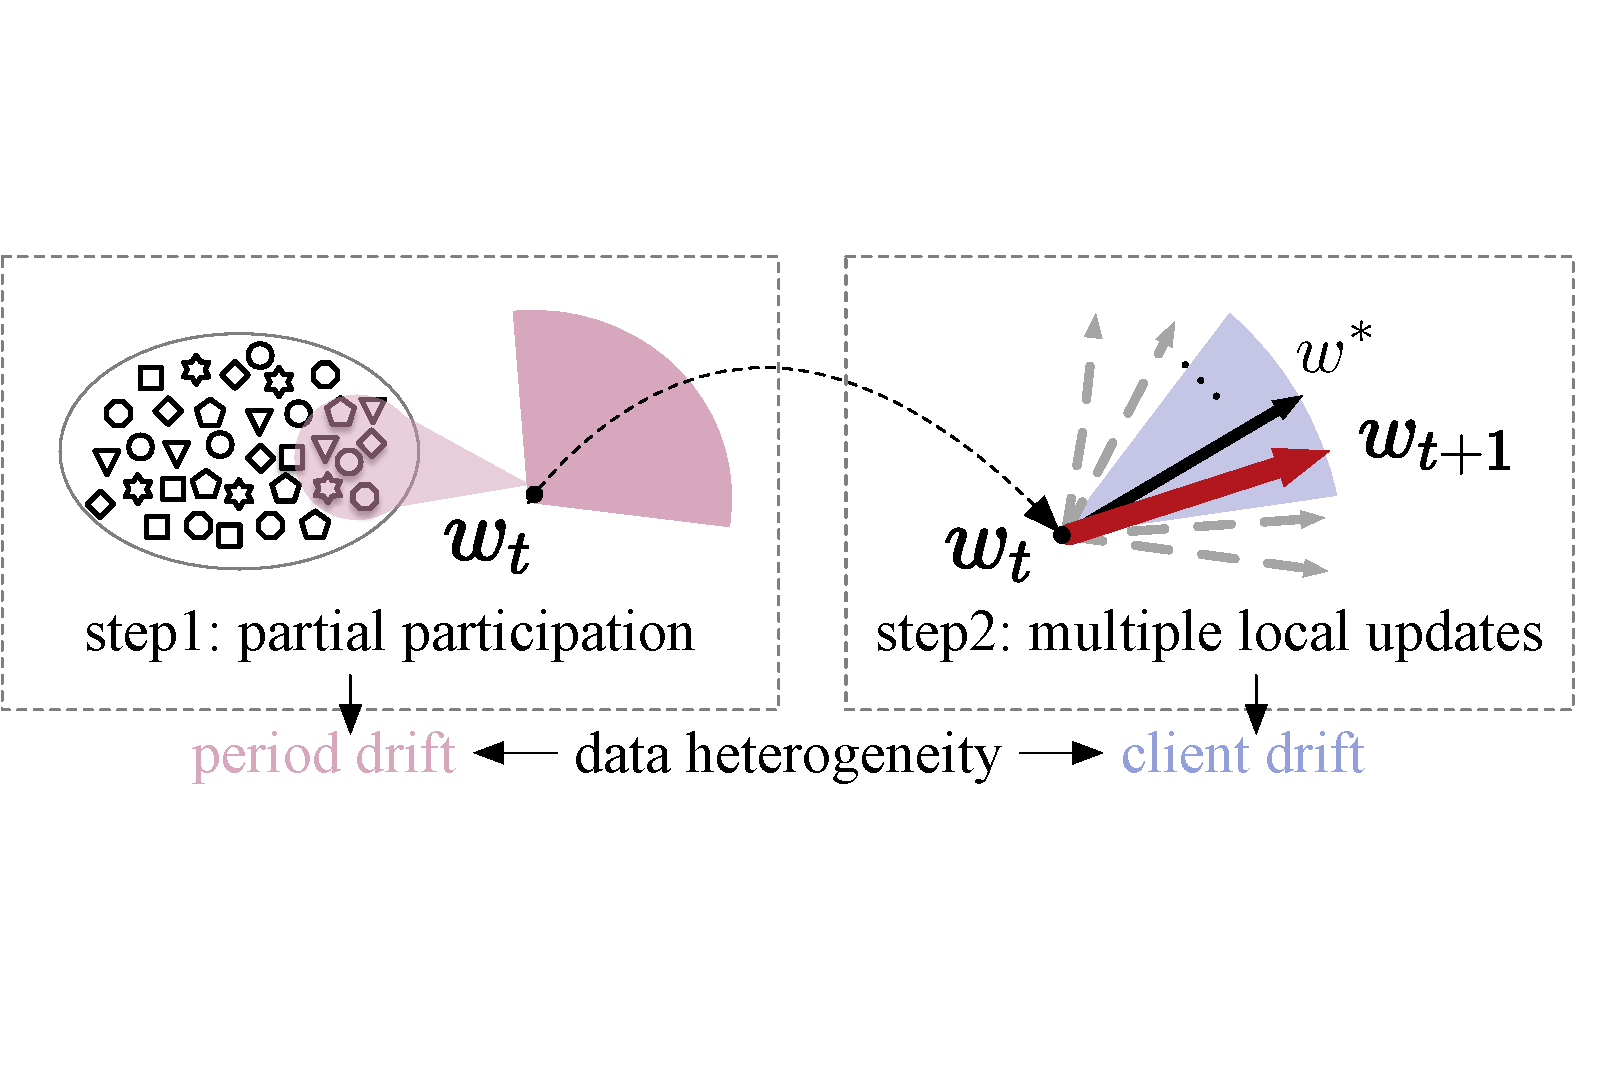
\includegraphics[width=0.55\textwidth]{illustration.pdf}
   \vspace{-3mm}
   \caption{\small\textbf{The generation of period drift and client drift}}
   \label{fig:illustration}
   \vspace{-3mm}
\end{wrapfigure}

This deviation could potentially lead to slow and unstable convergence, as the optimization objective shifts with every round. For simplicity, we refer to this phenomenon as \textit{\textbf{period drift}}. Despite both period drift and client drift being rooted in data heterogeneity, they stem from different causes (as illustrated in Figure~\ref{fig:illustration}). Client drift results from multiple local updates and the non-iid, while period drift arises due to partial client participation and the non-iid. 
The concept of period drift and client drift is shown in the following equation:\looseness-1

\begin{figure}[h]
   \vspace{-5mm}
\begin{equation}
   w^* \neq \tikzmarknode{wn}{w^* _ {\mathcal{N}}} \neq \tikzmarknode{ws}{w^* _ {\mathcal{S}}} \neq \tikzmarknode{wbar}{\bar{w}} =\frac{1}{|\mathcal{S}|}\sum w_k^*  \neq \tikzmarknode{wk}{w_k^*},
\end{equation}
   
   \begin{tikzpicture}[overlay,remember picture,>=stealth,nodes={align=left,inner ysep=1pt}]
       % Connect x_S* and x_N*
       \path (ws.south) ++ (-1em,-1.5em) node[anchor=north,color=PeriodDriftColor] (perioddrift){\textbf{Period Drift}};
       \draw[->,color=PeriodDriftColor] (ws.south) -- ++(0,-1.2em) -| (wn.south);
       % Connect average and x_k*
       \path (wk.south) ++ (-3.5em,-1.5em) node[anchor=north,color=ClientDriftColor] (clientdrift){\textbf{Client Drift}};
       \draw[->,color=ClientDriftColor] (wk.south) -- ++(0,-1.2em) -| (wbar.south);
   \end{tikzpicture}
\end{figure}
which is further described in detail in Appendix~\ref{appdx:concept}. These two drifts, when occurring simultaneously, significantly increase the complexity of achieving stable and efficient convergence, particularly challenging the effectiveness of cross-device FL systems.

%\vspace{1.5mm}
In this paper, we first investigate the impact of period drift and client drift, finding that period drift can have a particularly detrimental effect on cross-device FL as the degree of data heterogeneity increases (as demonstrated in detail in Section \ref{ex_period}). \textit{While the impacts of period drift and client drift are additive, we fortunately uncover a cooperative mechanism therby these two types of drift can compensate each other to mitigate their overall impact.} To achieve this, we propose a predict-observe framework, where we consider at each round 1) the server optimization (e.g., momentum) as a prediction of a update step of FL; 2) the clients' optimization (e.g., local SGD) as an observation of this update step. Note that the vanilla \fedavg is a special case in which the server does not make any predictions and solely relies on the observation provided by clients. In this framework, period drift and client drift are viewed as the noise respectively associated with prediction and observation. We thereby incorporate a Bayesian filter to integrate prediction (with period drift) and observation (with client drift) to achieve a better estimation of update step and reduce uncertainties. Based on the predict-observe framework, we present an instantiated method, referred as \fedeve, which combines the prediction and observation through linear interpolation. The coefficient of this linear combination indicate the relative confidence between prediction and observation, which is determined by the variance of the period drift and client drift, thus produces a more precise estimation of updates. \fedeve does not increase the client storage or extra communication costs, and does not introduce additional hyperparameter tunning, making it ideal for cross-device FL. 
% \footnote{For a smoother reading experience, please feel free to check out our reading guide in Appendix \ref{sec:reading_guide}.}

\textbf{Contributions} We summarize the primary contributions of this paper as follows:
\begin{itemize}[leftmargin=*,nosep]
   \item We analyze the impact of period drift and client drift for cross-device FL, and observe that period drift has a particularly detrimental effect as the degree of data heterogeneity increases.
   \item We propose a predict-observe framework for cross-device FL that incorporates a Bayesian filter to integrate server optimization and clients' optimization so that period drift and client drift can compensate for each other.
   \item As an instantiation of the proposed framework, we present \fedeve to combine prediction and observation through linear interpolation based on the variance of the period drift and client drift.
   \item We provide theoretical evidence within our framework that \fedeve can reduce the variance of model updates. Extensive experiments demonstrate that our method outperforms alternatives on non-iid data in cross-device settings. 
\footnote{For a smoother reading experience, please feel free to check out our reading guide in Appendix \ref{sec:reading_guide}.}
\end{itemize}




